\normallinespacing

\chapter{Introduction}
\section{Problem Statement}

Difficulty factors in games are rarely discussed as important, in this field of research the most normal topics of research are how to use the video games to learn or how to use video games with therapeutic purposes as we mentioned before in the abstract. In the video games field some games, they are well-thought-out additions, built for the hardcore players. Taking into account that the difficulty of a game is centered on the player and reflects his or her skills, these skills, therefore, change depending on the type of game or the condition of the player. For example: the skills used by a player who is used to playing shooting games may not be suitable for platforming games. Consequently, their score in a platforming game would also be lower considering that different reflexes and motor skills are needed. These are, of course, quite large suppositions, on which we will formulate our research question: What are the factors that affect the difficulty of video games for humans?, question we expect to resolve at the end of this research.

In this work, we will analyze the importance of different types of difficulty in video games to better understand what are the components that make video games hard or easy for humans. We chose video games as the task because many researchers are focused on solving video games but only a few of them are focused on humans. \cite{Dubey2018HumanPriors}

\section{State of the Art}
Why humans have a quick maturation when they play “hard” video games? Is the practice the only factor that makes this maturation faster? Which factors determine whether a video game is hard or easy for humans? We will try to address these questions and others as part of this research project. The idea is to go deeper into the difficulty of video games and their main components.  \cite{Dubey2018HumanPriors}

We will start with a short definition of the difficulty in video games and why it is important in the world of video games. Difficulty in video games is one of the most classic variables in this industry. From the difficulty levels to be selected by the game a priori, to the difficulty selectors in domestic video games.

Juul’s supports the importance of the difficulty in video games saying that: a game is a set of rules with a variable and quantifiable result when having to make an effort the player persists a challenge and foresees a direct influence of the difficulty in the result to be obtained. \cite{Aponte2009MeasuringDif}
On the other hand, Robin Hunicke describes a game as the use of Mechanics, Dynamics, and Aesthetics. The mechanics are the limits or rules created in a game, Dynamics are the possible interactions that the player generates based on the mechanics, and Aesthetics are the emotions generated in response by the player and it is perhaps the combination of these three components that it makes the difficulty continuously be perceived as a challenge to be overcome by the player. \cite{Aponte2009MeasuringDif}

After that, we must talk about video game difficulty. We need to separate difficulty into factors that make it hard or easy, such as reaction time, participant skills, attention limits (How many things on the game can I pay attention?), and physics in the virtual environment. As explained by Dubey (2018) some components in this area come from the context of the participant.  \cite{Dubey2018HumanPriors}

Imagine that you are playing a video game you have never played before, as shown in Figure 1(a). The game is well-known and the interactions are familiar to some humans (move in two directions, jump, use ladders to reach higher platforms, kill monsters and save the princess). The final goal is to rescue the princess by avoiding all the traps and enemies. This is a classic platforming game. 
The problem occurs when we change the visual stimulus for something less ordinary in the eyes of the human player (b), and a game that could take  2 minutes suddenly becomes a 10-minutes game or longer, which gives us the opportunity to analyze the factors that make it harder. In this research we are not focus on the human priors but for future research could be good to analyze this field too.
\cite{Dubey2018HumanPriors}



\begin{figure}[ht]
  \centering
  \begin{subfigure}[b]{0.45\linewidth}
    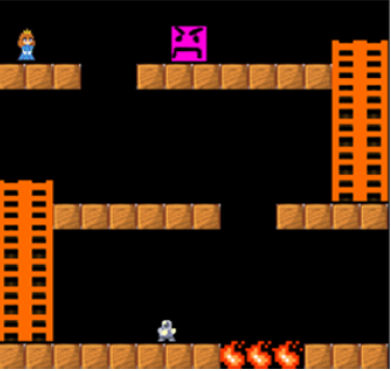
\includegraphics[width=\linewidth]{Figures/Example1a.png}
    \caption{Original State.}
  \end{subfigure}
  \begin{subfigure}[b]{0.45\linewidth}
    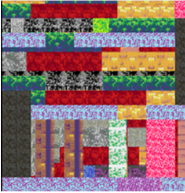
\includegraphics[width=\linewidth]{Figures/Example1b.png}
    \caption{Modified Game.}
  \end{subfigure}
  \caption{(a) A simple platformer game. (b) The same game modified by re-rendering the textures. Despite the two games being structurally the same, human players took twice as long to finish the second game as the first one. \cite{Dubey2018HumanPriors}}
  \label{fig:example}
\end{figure}

This paper will present a series of studies on a specially-designed game environment, The full game (unlike the first example) is going to be designed to be sufficiently complex for humans, taking into account the above mentioned factors, to easily measure the difficulty factors.

We are going to take the human as a logical being and test it on several settings where we vary such difficulty factors. It should be noted here that our aim is not to understand how humans learn a particular task (game) or how are they going to handle that task, but rather understand the entire process and to assess which types of task attributes affect human performance and how.

In addition to prior knowledge in this field (video games), humans also bring in rich prior knowledge about intuitive physics and strong motor control priors when they approach a new task. Here, one of our objectives is to take some initial steps to explore the importance of such priors in the context of humans into the difficulty in the video games field.

For us, that games that seem very different at first glance may be very similar at a more abstract level and beyond their immediate facade, games can be defined in terms of a number of factors, and furthermore it is these factors that define the complexity of a game and the best strategy to play it well.

-The factors mentioned above arise from the following questions:

-The number of players. Is the game played by a single player or multiple players, or does a single-player play with/against computer-controlled enemy units?

-Stochasticity. Is the outcome of the game determined only by the player?

-Time granularity. Is the game turn-based or real-time?

-Observability. Is the game partially observable or does the player have perfect information?

-Action space size. The number of actions the player can take.


In our case, we will analyze humans as the game-learners and consider games that can be played similarly to the ATARI 2600 games (Pac-Man, private eye, asteroids, etc...), where we can define and test the effect of such factors. Using average game scores, we will analyze the success of the task and how to perfect it. 
For instance, if the task is jumping on a vertically moving enemy, like in platforming game scores will depend on timing. If the jump is made at the right time, the score will be higher than if the jump is made out of time. In that way, we can assess the accuracy of the action in comparison with the skill being observed.

Within Damien Anderson's investigations, it can be seen how some artificial intelligence agents, when they are tested in some tasks, are vulnerable to several deceptions, so they can verify the weaknesses of several of these agents. If we use this logic with humans, ideally we might be able to discern other difficult factors for humans in video games and that can help us create new paradigms of difficulty. \cite{Anderson2018Deceptive}

At this point, we have used the term of difficulty in games without providing any definition of this word. We will not attempt to provide a general definition of difficulty covering a wide range of psychological aspects from emotional problems to intellectual and physical challenges. Instead, we consider the notion of difficulty in the sense used in game design, that is video games are built as combinations or sequences of predefined challenges. Thus, the study of the overall difficulty for a given video game involves studying the difficulty factors players experiment when overcoming a task. \cite{Aponte2011DifVideoGames}

In some cases games adapt the presented difficulty using the Dynamic Difficulty Adjustment (DDA). This is a general term used to express the change of difficulty during a game, it is a method to adapt the experience as the player's level increases. In the games that this method has been implemented, it is carried out starting from the adjustment of parameters, the modification of the level design, the automatic learning, the use of classification systems or the players modeling. \cite{Sarkar2019TransDif}

In the current investigation, we will not focus on AI, but further research could to compare these factors with AIs and humans, and analyzing if these difficulty factors affect both subjects. We estimate the AIs will present a better performance, yet also problems with some logical tasks like in Montezuma revenge or private eye or many others (ATARI 2600 games), According to some research, a very popular setting for a general-purpose evaluation today is the collection of games or tasks under an interactive scenario, where agents can perceive and act and are rewarded when they succeed. Many different platforms have recently appeared for that. Some benchmarks that have become particularly popular in the past years are the Arcade Learning Environment (ALE) and General Video Game Artificial Intelligence (GVGAI). \cite{Bontrager2019Superstition, Anderson2018Deceptive, Plumed2018DualIn}
%\section{Objectives}
%\section{Structure of the Report}


\newpage